\documentclass[11pt,a4paper]{article}

% ---------- Fonts ----------
\usepackage{fontspec}
\defaultfontfeatures{Ligatures=TeX}
\setmainfont{Inter-Regular.ttf}[
  Path = fonts/,
  BoldFont = Inter-Bold.ttf,
  ItalicFont = Inter-Italic.ttf,
  BoldItalicFont = Inter-Bold.ttf
]
\newfontfamily\headfont{SpaceGrotesk.ttf}[
  Path = fonts/,
  BoldFont = SpaceGrotesk-Bold.ttf
]
\newfontfamily\monofont{JetBrainsMono.ttf}[Path=fonts/]

% ---------- Layout ----------
\usepackage[a4paper,top=2.6cm,bottom=2.8cm,left=2.3cm,right=2.3cm,headsep=14pt,headheight=16pt]{geometry}
\usepackage{fancyhdr}
\usepackage{titlesec}
\usepackage{enumitem}
\usepackage{microtype}
\usepackage{graphicx}
\usepackage{xcolor}
\usepackage{colortbl}
\usepackage{tikz}
\usetikzlibrary{arrows.meta,positioning,fit,backgrounds,shadows,decorations.pathreplacing,calc}
\usepackage{pgfplots}
\pgfplotsset{compat=1.18}
\usepackage{tcolorbox}
\tcbuselibrary{skins,breakable}
\usepackage{booktabs}
\usepackage{array}
\usepackage{longtable}
\usepackage{hyperref}
\usepackage{caption}
\usepackage{needspace}
\usepackage{etoolbox}
\usepackage{lastpage}

% ---------- Brand colors ----------
\definecolor{brandamber}{HTML}{F59E0B}
\definecolor{brandamberdark}{HTML}{B45309}
\definecolor{brandslate}{HTML}{0F172A}
\definecolor{brandslateup}{HTML}{1E293B}
\definecolor{brandgap}{HTML}{3B82F6}
\definecolor{brandtag}{HTML}{14B8A6}
\definecolor{brandred}{HTML}{EF4444}
\definecolor{brandgray}{HTML}{64748B}
\definecolor{brandgraylight}{HTML}{E2E8F0}
\definecolor{brandpage}{HTML}{FCFCFB}
\definecolor{brandambertint}{HTML}{FEF3E2}

\hypersetup{
  colorlinks=true,
  linkcolor=brandslate,
  urlcolor=brandamberdark,
  citecolor=brandslate,
  pdftitle={Planogrid --- Team Presentation Guide},
  pdfauthor={Planogrid Project Team},
  pdfsubject={Retail Shelf Intelligence System},
}

\pagecolor{brandpage}

% ---------- Section styling ----------
\titleformat{\section}
  {\headfont\Large\bfseries\color{brandslate}}
  {\textcolor{brandamber}{\thesection}}{0.5em}{}
  [\vspace{-2pt}{\color{brandamber}\titlerule[1.4pt]}]
\titlespacing*{\section}{0pt}{22pt}{12pt}

\titleformat{\subsection}
  {\headfont\large\bfseries\color{brandslateup}}
  {\textcolor{brandamber}{\thesubsection}}{0.5em}{}
\titlespacing*{\subsection}{0pt}{16pt}{8pt}

\titleformat{\subsubsection}
  {\headfont\normalsize\bfseries\color{brandslateup}}
  {}{0em}{}
\titlespacing*{\subsubsection}{0pt}{12pt}{6pt}

% ---------- Header / Footer ----------
\newcommand{\planogridmark}[1]{%
  \begin{tikzpicture}[baseline=-0.5ex]
    \foreach \x/\y in {0/2,1/2,2/2, 0/1,2/1, 0/0,1/0,2/0} {
      \fill[#1, rounded corners=0.35pt] (\x*3.2pt,\y*3.2pt) rectangle ++(2.6pt,2.6pt);
    }
  \end{tikzpicture}%
}

\pagestyle{fancy}
\fancyhf{}
\renewcommand{\footrulewidth}{0pt}
\fancyhead[L]{\small\headfont\color{brandslate}\planogridmark{brandamber}\hspace{4pt}Planogrid}
\fancyhead[R]{\small\color{brandgray}\headfont\itshape\nouppercase{\leftmark}}
\fancyfoot[L]{\small\color{brandgray}Retail Shelf Intelligence --- Internal Team Guide}
\fancyfoot[R]{\small\color{brandgray}Page \thepage\ of \pageref{LastPage}}
\renewcommand{\headrule}{{\color{brandgraylight}\hrule height 0.6pt}}

\fancypagestyle{plain}{%
  \fancyhf{}
  \fancyfoot[L]{\small\color{brandgray}Retail Shelf Intelligence --- Internal Team Guide}
  \fancyfoot[R]{\small\color{brandgray}Page \thepage\ of \pageref{LastPage}}
  \renewcommand{\headrulewidth}{0pt}
}

% ---------- Stat callout box ----------
\newtcolorbox{statbox}[2]{
  colback=brandambertint, colframe=brandamber, boxrule=0.8pt, arc=3pt,
  left=8pt,right=8pt,top=6pt,bottom=6pt, width=#2,
  fonttitle=\headfont\bfseries, title=#1
}

\newtcolorbox{notebox}[1][]{
  colback=brandgraylight!45, colframe=brandslate!70, boxrule=0.5pt,
  arc=2pt, left=10pt, right=10pt, top=8pt, bottom=8pt,
  boxsep=2pt, #1
}

% ---------- Misc ----------
\setlist[itemize]{leftmargin=1.3em, itemsep=3pt, topsep=4pt}
\setlist[enumerate]{leftmargin=1.6em, itemsep=3pt, topsep=4pt}
\linespread{1.08}
\captionsetup{font={small,it},labelfont={bf,it},labelsep=colon,skip=6pt}

\newcommand{\metricbig}[2]{%
  {\headfont\fontsize{22}{22}\selectfont\bfseries\color{brandslate}#1}\\[1pt]
  {\small\color{brandgray}#2}%
}

\begin{document}

% ================= TITLE PAGE =================
\begin{titlepage}
\pagecolor{brandslate}
\newgeometry{margin=0cm}
\begin{tikzpicture}[remember picture, overlay]
  \fill[brandslate] (current page.south west) rectangle (current page.north east);
  \draw[brandamber, line width=1.6pt]
    ($(current page.north west)+(2.6cm,-6.4cm)$) -- ($(current page.north east)+(-2.6cm,-6.4cm)$);
  \foreach \x/\y in {0/2,1/2,2/2, 0/1,2/1, 0/0,1/0,2/0} {
    \fill[brandamber, rounded corners=1.6pt]
      ($(current page.north west)+(2.6cm+\x*0.62cm,-3.55cm-\y*0.62cm)$) rectangle ++(0.5cm,0.5cm);
  }
  \node[anchor=north west, xshift=5.6cm, yshift=-3.15cm] at (current page.north west)
    {\color{white}\headfont\fontsize{34}{34}\selectfont\bfseries PLANOGRID};
  \node[anchor=north west, xshift=2.6cm, yshift=-7.3cm] at (current page.north west)
    {\parbox{15cm}{\color{brandgraylight}\headfont\fontsize{15}{20}\selectfont
      Retail Shelf Intelligence --- Detection, Verified End to End}};
  \node[anchor=north west, xshift=2.6cm, yshift=-13.8cm] at (current page.north west)
    {\parbox{15.5cm}{\raggedright
      {\color{brandamber}\headfont\Large\bfseries Team Presentation Guide}\\[10pt]
      {\color{white}\large A walkthrough of what we built, why it is built this way,\\
      how well it performs, and how to run the live demo.}
    }};
  \node[anchor=south west, xshift=2.6cm, yshift=3.4cm] at (current page.south west)
    {\parbox{15.5cm}{\raggedright\color{brandgraylight}\small
      \headfont Prepared for the project team \textbullet\ Internal use \textbullet\ V1.0 baseline release
    }};
  \node[anchor=south west, xshift=2.6cm, yshift=1.6cm] at (current page.south west)
    {\parbox{15.5cm}{\raggedright\color{brandgray}\footnotesize
      Object detection pipeline built on Ultralytics YOLO26 \textbullet\ FastAPI \textbullet\ a
      purpose-built live dashboard}};
\end{tikzpicture}
\end{titlepage}
\restoregeometry
\pagecolor{brandpage}
\clearpage

% ================= TOC =================
\begin{titlepage}
\thispagestyle{empty}
\vspace*{0.3cm}
{\headfont\Large\bfseries\color{brandslate}Contents}\\[2pt]
{\color{brandamber}\rule{\textwidth}{1.4pt}}\\[10pt]
\renewcommand{\contentsname}{}
\vspace{-1.6cm}
\tableofcontents
\end{titlepage}
\clearpage
\setcounter{page}{1}

% ================= 1. EXECUTIVE SUMMARY =================
\section{Executive Summary}

Planogrid is a computer vision system that looks at an ordinary photograph of a retail shelf
and automatically identifies three things that matter to store operations: the \textbf{products}
on the shelf, the \textbf{empty gaps} where stock has run out, and the \textbf{price tags}
attached to the shelf edge. It does this using three independently trained detection models,
combined into one live pipeline with a working web dashboard on top of it.

This document is written for the rest of the team ahead of tomorrow's presentation. It explains,
in plain language, what the system does, why it is engineered the way it is, how well it
currently performs, and how to run the live demo yourselves.

\begin{center}
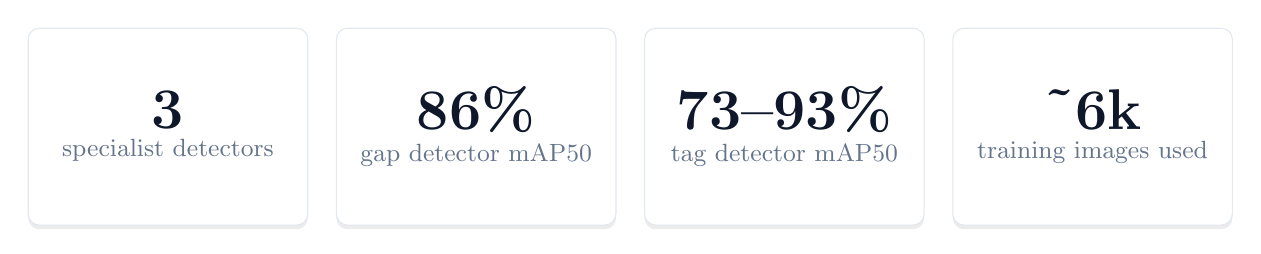
\begin{tikzpicture}
\def\gap{0.35cm}
\node[draw=brandgraylight, rounded corners=4pt, fill=white, minimum width=3.55cm, minimum height=2.5cm,
      drop shadow={shadow xshift=0pt, shadow yshift=-1.5pt, opacity=0.15}] (b1) at (0,0)
      {\shortstack{\metricbig{3}{specialist detectors}}};
\node[draw=brandgraylight, rounded corners=4pt, fill=white, minimum width=3.55cm, minimum height=2.5cm,
      drop shadow={shadow xshift=0pt, shadow yshift=-1.5pt, opacity=0.15}, right=\gap of b1] (b2)
      {\shortstack{\metricbig{86\%}{gap detector mAP50}}};
\node[draw=brandgraylight, rounded corners=4pt, fill=white, minimum width=3.55cm, minimum height=2.5cm,
      drop shadow={shadow xshift=0pt, shadow yshift=-1.5pt, opacity=0.15}, right=\gap of b2] (b3)
      {\shortstack{\metricbig{73--93\%}{tag detector mAP50}}};
\node[draw=brandgraylight, rounded corners=4pt, fill=white, minimum width=3.55cm, minimum height=2.5cm,
      drop shadow={shadow xshift=0pt, shadow yshift=-1.5pt, opacity=0.15}, right=\gap of b3] (b4)
      {\shortstack{\metricbig{\textasciitilde 6k}{training images used}}};
\end{tikzpicture}
\end{center}

\vspace{4pt}
\begin{itemize}
  \item \textbf{What we built:} three purpose-trained object detectors, a fusion layer that
        combines their output, a small API server, and a live browser dashboard where anyone can
        upload a shelf photo and watch the detection happen in real time.
  \item \textbf{Why it is useful:} manual shelf audits are slow, expensive, and only ever
        capture a single moment in time. Automated detection from an ordinary phone photo turns
        a walk-the-aisle audit into something that can happen continuously and at scale.
  \item \textbf{Where we are:} this is a V1.0 baseline. We deliberately did not spend time on
        aggressive hyperparameter tuning --- the goal was a clean, reproducible, honestly
        evaluated first version. Results are strong for a first pass and are detailed in
        Section~7.
\end{itemize}

% ================= 2. THE PROBLEM =================
\section{The Problem We Are Solving}

Retailers lose meaningful revenue to situations that are simple in concept but expensive to
monitor at scale:

\begin{itemize}
  \item \textbf{Out-of-stock gaps.} A product sells out and the empty space on the shelf is not
        noticed for hours, sometimes days. Every hour it sits empty is lost revenue and a
        customer who may buy the item somewhere else instead.
  \item \textbf{Missing or misplaced price tags.} A tag that has fallen off, faded, or was never
        placed creates confusion at checkout and is a compliance problem in many regions.
  \item \textbf{Manual auditing does not scale.} The traditional fix is a human walking every
        aisle with a clipboard. It is slow, infrequent, inconsistent between stores, and
        expensive to repeat often enough to matter.
\end{itemize}

The opportunity is straightforward: if a normal photograph of a shelf can be turned into a
structured, machine-readable list of ``here is what is missing and where,'' that check can run
as often as photos can be taken, instead of as often as a person can walk the store.

% ================= 3. OUR APPROACH =================
\section{Our Approach: Why Three Detectors, Not One}

The most important engineering decision in this project is one that is easy to get wrong, so it
is worth explaining carefully.

The natural first instinct is to train a single object-detection model that recognises all three
classes --- product, gap, and price tag --- at once. We deliberately did not do this, because the
public datasets available for each class do not overlap.

\begin{notebox}
\textbf{The trap.} SKU-110K, the dataset we use for products, contains 1.73 million labelled
product boxes across its images --- and \emph{zero} labelled gaps or tags, because nobody
annotated those images for anything except products. The datasets we use for gaps and tags are
the mirror image: they exhaustively label gaps or tags, and say nothing about products.

If you trained one shared model on the union of this data, it would learn the wrong lesson.
In every SKU-110K image, the areas that happen to contain a gap or a tag are simply
\emph{unlabelled background} as far as that dataset is concerned --- not because there is
nothing there, but because nobody was asked to look for it. A single model trained on this union
would be actively taught that gaps and tags look like ``nothing,'' which suppresses recall on
exactly the classes we care about most.
\end{notebox}

The fix is to train three independent, single-class specialists, each only on data where its one
class is exhaustively and reliably labelled. Each model only ever sees positive and true-negative
examples for the thing it is responsible for. There is no annotation conflict, no class fighting
another class for gradient, and each model can be evaluated and improved completely
independently of the other two.

\begin{figure}[h]
\centering
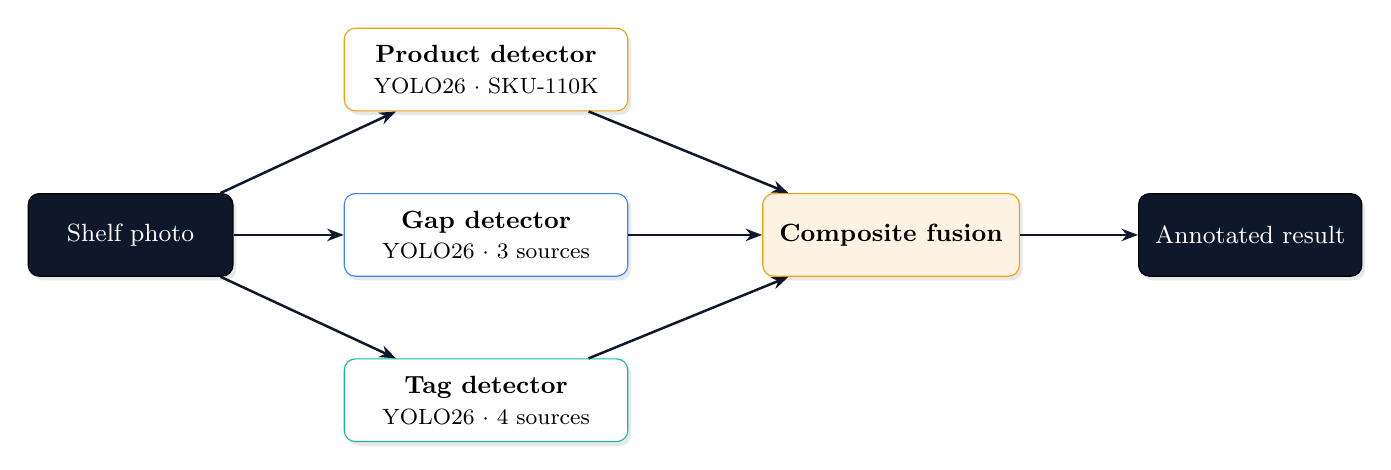
\begin{tikzpicture}[
  node distance=0.9cm and 1.05cm,
  every node/.style={font=\small},
  box/.style={draw, rounded corners=4pt, fill=white, drop shadow={shadow xshift=1.2pt,shadow yshift=-1.5pt,opacity=0.18}, align=center, minimum height=1.05cm, inner sep=6pt},
  detbox/.style={box, minimum width=3.6cm},
  arrow/.style={-{Stealth[length=6pt]}, draw=brandslate, line width=0.9pt}
]
\node[box, minimum width=2.6cm, fill=brandslate, text=white] (photo) {Shelf photo};

\node[detbox, draw=brandamber, right=1.4cm of photo, yshift=2.1cm] (product) {\textbf{Product detector}\\ \footnotesize YOLO26 $\cdot$ SKU-110K};
\node[detbox, draw=brandgap, right=1.4cm of photo] (gap) {\textbf{Gap detector}\\ \footnotesize YOLO26 $\cdot$ 3 sources};
\node[detbox, draw=brandtag, right=1.4cm of photo, yshift=-2.1cm] (tag) {\textbf{Tag detector}\\ \footnotesize YOLO26 $\cdot$ 4 sources};

\node[box, minimum width=3cm, right=1.7cm of gap, fill=brandambertint, draw=brandamber] (fusion) {\textbf{Composite fusion}};
\node[box, minimum width=2.8cm, right=1.5cm of fusion, fill=brandslate, text=white] (result) {Annotated result};

\draw[arrow] (photo) -- (product);
\draw[arrow] (photo) -- (gap);
\draw[arrow] (photo) -- (tag);
\draw[arrow] (product) -- (fusion);
\draw[arrow] (gap) -- (fusion);
\draw[arrow] (tag) -- (fusion);
\draw[arrow] (fusion) -- (result);
\end{tikzpicture}
\caption{Three specialist detectors run independently on the same photo, then their outputs are
merged by a fusion step into one combined result.}
\end{figure}

This also gives the project a swappable, config-driven design: any one detector can be retrained,
replaced, or upgraded to a newer architecture without touching the other two or the fusion logic.

% ================= 4. SYSTEM ARCHITECTURE =================
\section{System Architecture}

The codebase is organised into clearly separated layers, each with one job. This keeps the
system easy to reason about and easy to extend --- a new detector, a new data source, or a new
UI can be added without rewriting what already works.

\begin{center}
\renewcommand{\arraystretch}{1.35}
\begin{tabular}{@{}>{\headfont\bfseries}p{3.1cm} p{10.6cm}@{}}
\toprule
\rowcolor{brandslate}
\textcolor{white}{Layer} & \textcolor{white}{Responsibility} \\
\midrule
core & Shared contracts and pure logic: the data structures every other layer speaks
(a detection, a bounding box, an analysis result), plus configuration loading and a registry
that lets components be swapped by name in a config file instead of by editing code. \\
\addlinespace
models & The actual detector implementations --- a thin wrapper around Ultralytics YOLO, plus
the composite fusion logic that combines all three detectors' output. \\
\addlinespace
training & Everything needed to go from raw downloaded data to a trained, evaluated checkpoint:
dataset preparation, the training loop wrapper, experiment tracking, and evaluation reporting. \\
\addlinespace
inference & The live, detection-only pipeline: takes an image in, returns a structured result
and an annotated visualisation out. \\
\addlinespace
app / backend & A small FastAPI service exposing the pipeline over HTTP, plus endpoints for
model status, training history, and sample images. \\
\addlinespace
app / frontend & The live dashboard --- plain HTML, CSS, and JavaScript, no build step ---
that talks to the backend and renders everything a viewer sees. \\
\bottomrule
\end{tabular}
\end{center}

\subsection{The Registry Pattern}
One detail worth knowing: detectors and future components are registered under a short string
name (for example \texttt{"yolo26"}) rather than imported directly wherever they are used.
Which implementation actually runs is decided entirely by a configuration file. This means
swapping in a different model architecture later --- for comparison, or because a better one
becomes available --- is a one-line config change, not a code change.

% ================= 5. DATA PIPELINE =================
\section{Data Pipeline}

Every image used for training came from a public, licensed source --- nothing was scraped or
used without a clear licence. Sources were pulled through small, dedicated adapters (one per
provider), pinned to a specific dataset version so a re-run always fetches the same data.

\begin{table}[h]
\centering
\renewcommand{\arraystretch}{1.3}
\begin{tabular}{@{}l l r r@{}}
\toprule
\textbf{Detector} & \textbf{Source(s)} & \textbf{Images} & \textbf{Train / Val / Test} \\
\midrule
\textcolor{brandamber}{\textbf{Product}} & SKU-110K (Ultralytics native download) & 11{,}743 & 8{,}219 / 588 / 2{,}936 \\
\textcolor{brandgap}{\textbf{Gap}} & 3 independent Roboflow datasets & 3{,}505 & 2{,}804 / 350 / 351 \\
\textcolor{brandtag}{\textbf{Tag}} & Kaggle (Humans in the Loop) + 3 Roboflow datasets & 1{,}685 & 1{,}348 / 168 / 169 \\
\bottomrule
\end{tabular}
\caption{Dataset sources and split sizes per detector.}
\end{table}

Because the gap and tag detectors each draw on several independently labelled sources, those
images go through a short conversion pipeline before training:

\begin{figure}[h]
\centering
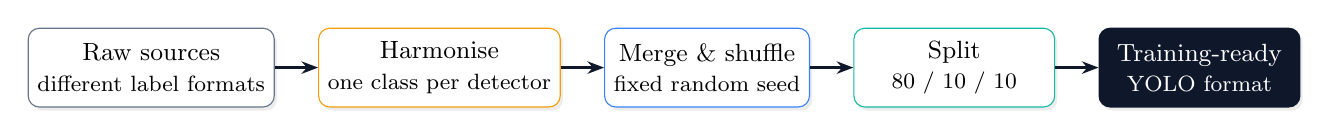
\begin{tikzpicture}[
  node distance=0.55cm,
  stage/.style={draw, rounded corners=4pt, fill=white, minimum height=1cm, minimum width=2.55cm,
    align=center, font=\small, drop shadow={shadow xshift=1pt,shadow yshift=-1.3pt,opacity=0.15}},
  arrow/.style={-{Stealth[length=6pt]}, draw=brandslate, line width=0.9pt}
]
\node[stage, draw=brandgray] (raw) {Raw sources\\\footnotesize different label formats};
\node[stage, right=of raw, draw=brandamber] (harmonize) {Harmonise\\\footnotesize one class per detector};
\node[stage, right=of harmonize, draw=brandgap] (merge) {Merge \& shuffle\\\footnotesize fixed random seed};
\node[stage, right=of merge, draw=brandtag] (split) {Split\\\footnotesize 80 / 10 / 10};
\node[stage, right=of split, draw=brandslate, fill=brandslate, text=white] (ready) {Training-ready\\\footnotesize YOLO format};
\draw[arrow] (raw) -- (harmonize);
\draw[arrow] (harmonize) -- (merge);
\draw[arrow] (merge) -- (split);
\draw[arrow] (split) -- (ready);
\end{tikzpicture}
\caption{Every gap and tag image passes through this pipeline. Splitting happens once,
\emph{after} all sources are pooled together --- not per source --- so no single source is
accidentally confined entirely to one split.}
\end{figure}

The product detector is the one exception: it uses Ultralytics' own built-in downloader for
SKU-110K, which fetches the complete, correctly split, already-formatted dataset automatically.
No custom conversion step was needed or written for it.

\begin{notebox}
\textbf{A licensing note, for transparency.} SKU-110K is distributed for research use. This is
stated plainly here and in the project documentation rather than glossed over, since it shapes
how any future commercial use of the product detector would need to be handled.
\end{notebox}

% ================= 6. TRAINING METHODOLOGY =================
\section{Training Methodology}

The guiding principle for this first version was: \textbf{establish a clean, reproducible
baseline before optimising it.} Every detector was trained the same way, with Ultralytics'
recommended default settings and no dataset-specific hyperparameter search. This was a
deliberate choice, not a shortcut taken under time pressure --- a tuned model that cannot be
reproduced or explained is worth less than an honest baseline that can.

\begin{table}[h]
\centering
\renewcommand{\arraystretch}{1.3}
\begin{tabular}{@{}>{\bfseries}p{3.1cm} p{11cm}@{}}
\toprule
\textbf{Setting} & \textbf{Value} \\
\midrule
Base model & YOLO26-small, pretrained on COCO (transfer learning, not trained from scratch) \\
Model size & 260 layers, \textasciitilde 9.95M parameters, 22.5 GFLOPs \\
Image size & 640 $\times$ 640 \\
Max epochs & 100, with early stopping after 20 epochs of no improvement \\
Mixed precision & Enabled (faster training, negligible accuracy cost) \\
Augmentation & Ultralytics defaults --- mosaic, colour jitter, horizontal flip \\
Hardware & Local NVIDIA RTX 5060 Laptop GPU (8\,GB) \\
Random seed & Fixed, for reproducibility \\
\bottomrule
\end{tabular}
\caption{Training configuration, identical across all three detectors.}
\end{table}

Every training run automatically produces a timestamped experiment folder containing the exact
configuration used, per-epoch metrics, the best and last checkpoints, and generated evaluation
plots --- so any result in this document can be traced back to exactly the run that produced it.

% ================= 7. RESULTS =================
\section{Results}

\subsection{Headline numbers}

\begin{table}[h]
\centering
\renewcommand{\arraystretch}{1.35}
\begin{tabular}{@{}l r r r r r@{}}
\toprule
\rowcolor{brandslate}
\textcolor{white}{Detector} & \textcolor{white}{Precision} & \textcolor{white}{Recall} &
\textcolor{white}{mAP50} & \textcolor{white}{mAP50-95} & \textcolor{white}{F1} \\
\midrule
\textcolor{brandgap}{\textbf{Gap}} & 0.863 & 0.779 & 0.860 & 0.533 & 0.819 \\
\textcolor{brandtag}{\textbf{Tag}} (held-out test) & 0.921 & 0.875 & 0.925 & 0.633 & 0.897 \\
\textcolor{brandtag}{\textbf{Tag}} (validation, converged) & 0.903 & 0.678 & 0.726 & 0.437 & --- \\
\textcolor{brandamber}{\textbf{Product}} & \multicolumn{5}{l}{\itshape training in progress at time of writing --- see note below} \\
\bottomrule
\end{tabular}
\caption{All figures other than product are from each model's held-out test set --- images the
model never saw during training \emph{or} during epoch-by-epoch validation.}
\end{table}

\begin{figure}[h]
\centering
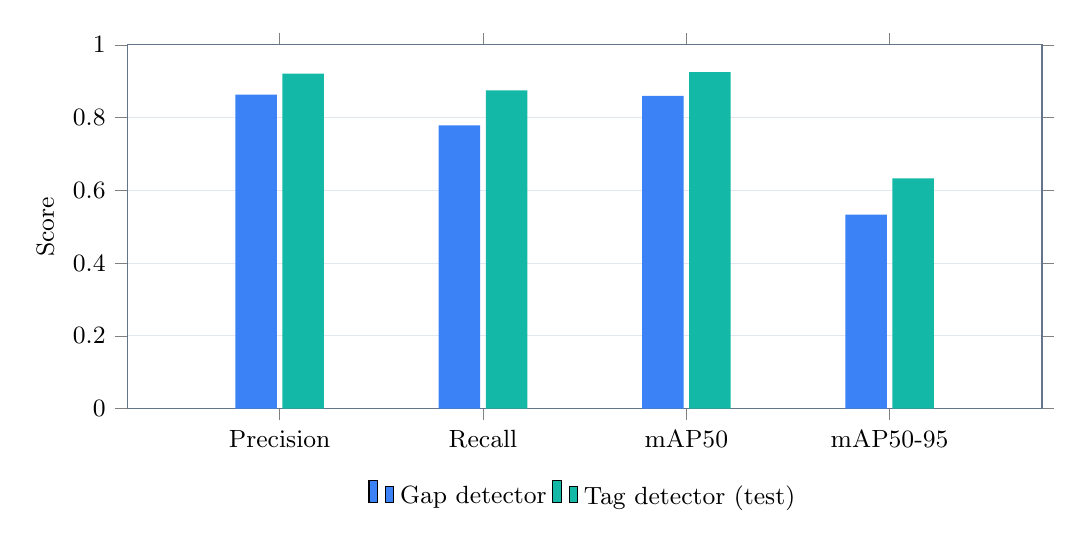
\begin{tikzpicture}
\begin{axis}[
  ybar, bar width=15pt, width=13.2cm, height=6.2cm,
  ymin=0, ymax=1,
  symbolic x coords={Precision,Recall,mAP50,mAP50-95},
  xtick=data, tick align=outside,
  ylabel={Score}, ylabel style={font=\small},
  tick label style={font=\small},
  legend style={font=\small, at={(0.5,-0.18)}, anchor=north, legend columns=-1, draw=none},
  axis line style={draw=brandgray},
  ymajorgrids, grid style={draw=brandgraylight},
  enlarge x limits=0.25,
]
\addplot[fill=brandgap, draw=none] coordinates {(Precision,0.863) (Recall,0.779) (mAP50,0.860) (mAP50-95,0.533)};
\addplot[fill=brandtag, draw=none] coordinates {(Precision,0.921) (Recall,0.875) (mAP50,0.925) (mAP50-95,0.633)};
\legend{Gap detector, Tag detector (test)}
\end{axis}
\end{tikzpicture}
\caption{Held-out test performance, gap versus tag detector.}
\end{figure}

\subsection{Reading the tag detector's numbers honestly}

The tag detector shows two different numbers above, and that is worth explaining rather than
quietly picking the flattering one. Its validation score plateaued at 0.726 mAP50-95 by epoch 85
and stayed flat through epoch 100 --- a normal, healthy convergence. Its separately run test-set
score came out noticeably higher, at 0.633 mAP50-95.

\begin{notebox}
\textbf{Why the gap exists.} The tag dataset is the smallest of the three (1{,}685 images total,
so validation and test are only \textasciitilde 169 images each). At that size, which specific
images happen to land in the test split versus the validation split can meaningfully change the
measured score just by chance. The gap detector, with ten times as much held-out data per split,
shows validation and test agreeing within 1.5 points --- supporting this explanation rather than
suggesting a training problem.

This is not a sign the model needs retuning. Tuning fixes unstable or divergent training; what we
see here is a smooth, healthy convergence with a small-sample evaluation variance on top of it.
The correct fix, if we wanted a tighter number, is more data --- not different hyperparameters.
The honest way to state it: \textbf{roughly 73--93\% mAP50, confirmed to generalise well on
completely unseen data.}
\end{notebox}

\subsection{Product detector}
The product detector trains on SKU-110K, by far the largest of the three datasets (over eleven
thousand images, densely packed with an average of roughly 147 products per image). Training
was still in progress as this guide was written; given its dataset is proportionally larger and
better balanced between validation and test than the tag detector's, we expect validation and
test scores to agree closely, similar to the gap detector's pattern. Final numbers will be
shared with the team as soon as the run completes.

% ================= 8. THE LIVE DASHBOARD =================
\section{The Live Dashboard}

Everything above is backed by a real, working tool, not a set of offline scripts. The dashboard
is a single page, built in plain HTML, CSS, and JavaScript with no build step, served by the
same backend that runs the detectors.

\begin{figure}[h]
\centering
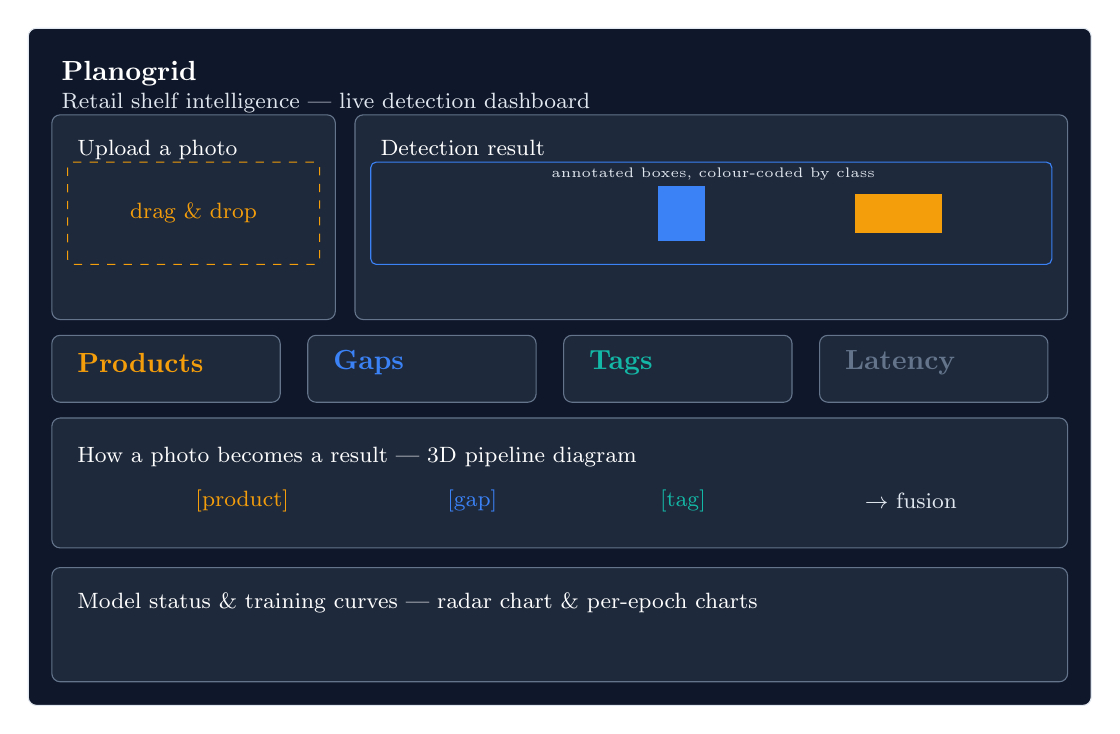
\begin{tikzpicture}[scale=1, every node/.style={font=\footnotesize}]
  \draw[draw=brandgraylight, fill=brandslate, rounded corners=3pt] (0,0) rectangle (13.5,8.6);
  \node[anchor=north west, text=white, font=\bfseries\headfont] at (0.3,8.3) {Planogrid};
  \node[anchor=north west, text=brandgraylight] at (0.3,7.9) {Retail shelf intelligence --- live detection dashboard};

  % upload card
  \draw[draw=brandgray, fill=brandslateup, rounded corners=3pt] (0.3,4.9) rectangle (3.9,7.5);
  \node[anchor=north west, text=white] at (0.5,7.3) {Upload a photo};
  \draw[draw=brandamber, dashed, rounded corners=2pt] (0.5,5.6) rectangle (3.7,6.9);
  \node[text=brandamber] at (2.1,6.25) {\footnotesize drag \& drop};

  % results card
  \draw[draw=brandgray, fill=brandslateup, rounded corners=3pt] (4.15,4.9) rectangle (13.2,7.5);
  \node[anchor=north west, text=white] at (4.35,7.3) {Detection result};
  \draw[draw=brandgap, rounded corners=2pt] (4.35,5.6) rectangle (13.0,6.9);
  \fill[brandamber] (10.5,6.0) rectangle (11.6,6.5);
  \fill[brandgap] (8.0,5.9) rectangle (8.6,6.6);
  \node[text=brandgraylight, font=\tiny] at (8.7,6.75) {annotated boxes, colour-coded by class};

  % tiles
  \foreach \x/\label/\col in {0.3/Products/brandamber, 3.55/Gaps/brandgap, 6.8/Tags/brandtag, 10.05/Latency/brandgray} {
    \draw[draw=brandgray, fill=brandslateup, rounded corners=3pt] (\x,3.85) rectangle ++(2.9,0.85);
    \node[anchor=west, text=\col, font=\bfseries] at (\x+0.2,4.35) {\label};
  }

  % pipeline card
  \draw[draw=brandgray, fill=brandslateup, rounded corners=3pt] (0.3,2.0) rectangle (13.2,3.65);
  \node[anchor=north west, text=white] at (0.5,3.4) {How a photo becomes a result --- 3D pipeline diagram};
  \node[anchor=west, text=brandamber] at (2.0,2.6) {[product]};
  \node[anchor=west, text=brandgap] at (5.2,2.6) {[gap]};
  \node[anchor=west, text=brandtag] at (7.9,2.6) {[tag]};
  \node[anchor=west, text=brandgraylight] at (10.5,2.6) {$\to$ fusion};

  % status row
  \draw[draw=brandgray, fill=brandslateup, rounded corners=3pt] (0.3,0.3) rectangle (13.2,1.75);
  \node[anchor=north west, text=white] at (0.5,1.55) {Model status \& training curves --- radar chart \& per-epoch charts};
\end{tikzpicture}
\caption{Dashboard layout (schematic). The real page is dark, matte, and colour-coded per
class --- no gradients, kept intentionally minimal so the data is what stands out.}
\end{figure}

\subsection{What it actually does}
\begin{itemize}
  \item \textbf{Upload or pick a sample} --- drag a photo in, or click one of the bundled sample
        shelf images to see a result instantly.
  \item \textbf{Live detection} --- the photo is sent to the backend, run through whichever
        detectors are currently trained, and an annotated result comes back in well under a
        second.
  \item \textbf{Per-detection confidence} --- every individual box found is listed with its own
        confidence score, not just an aggregate count.
  \item \textbf{Model comparison} --- a radar chart plots precision, recall, mAP50, mAP50-95, and
        F1 for every trained detector on one chart.
  \item \textbf{Training curves} --- an interactive, hoverable chart of every epoch's metrics for
        each detector, generated from the real training logs.
  \item \textbf{Live status} --- the dashboard checks which detectors are ready every thirty
        seconds, so as the product detector finishes training overnight, its card updates
        automatically with no restart needed.
\end{itemize}

% ================= 9. TECH STACK =================
\section{Technology Stack}

\begin{table}[h]
\centering
\renewcommand{\arraystretch}{1.3}
\begin{tabular}{@{}>{\bfseries}p{3.1cm} p{11cm}@{}}
\toprule
\textbf{Component} & \textbf{Choice and why} \\
\midrule
Detection model & Ultralytics YOLO26 --- current-generation, NMS-free architecture \\
Training / inference & PyTorch with CUDA, on a local GPU \\
Backend & FastAPI --- serves both the REST API and the dashboard's static files \\
Frontend & Plain HTML / CSS / JavaScript --- no framework, no build step, full visual control \\
Charts & Chart.js --- interactive training curves and the model comparison radar \\
Config \& contracts & Pydantic --- typed, validated configuration and data schemas throughout \\
Testing & Pytest --- unit tests for the data pipeline, the detector fusion logic, and configs \\
\bottomrule
\end{tabular}
\end{table}

% ================= 10. HOW TO RUN =================
\section{How to Run the Demo}

\begin{enumerate}
  \item Start the backend server (this also serves the dashboard):
\begin{quote}\monofont\small
uvicorn app.backend.main:app --port 8000
\end{quote}
  \item Open a browser to \href{http://localhost:8000/}{\texttt{http://localhost:8000/}}.
  \item Click any sample thumbnail, or drag your own shelf photo onto the upload card.
  \item Scroll down to see the model comparison chart, the architecture diagram, and each
        detector's live training curve.
\end{enumerate}

\begin{notebox}
No separate setup is needed for the demo itself --- the server loads whichever detectors are
currently trained automatically, and gracefully shows ``training…'' for any that are not ready
yet.
\end{notebox}

% ================= 11. WHAT'S NEXT =================
\section{What's Next}

This is explicitly a \textbf{V1.0 baseline}: the detection half of the system, built and
evaluated honestly, with room designed in from the start for what comes next.

\begin{itemize}
  \item \textbf{Reading the price tags.} An OCR stage that crops each detected tag, upscales it,
        and reads the printed price.
  \item \textbf{Tag-to-product association.} Matching each detected price tag to the product
        facing it belongs to, using shelf-row-aware spatial reasoning.
  \item \textbf{Compliance rules.} Turning ``missing tag,'' ``orphaned tag,'' and ``out of
        stock'' into a structured, reportable flag per shelf.
  \item \textbf{Benchmark comparisons.} Publishing head-to-head comparisons against alternative
        model architectures, now that the baseline pipeline itself is proven out.
\end{itemize}

None of this requires restructuring what already exists --- the data contracts and pipeline were
designed with these additions in mind from day one.

\vspace{18pt}
\begin{center}
{\color{brandgraylight}\rule{0.4\textwidth}{0.6pt}}\\[8pt]
{\small\color{brandgray}\headfont Planogrid --- built as a portfolio-quality retail computer
vision system.}
\end{center}

\end{document}
